%

% File final_report.tex
%
%% Based on the style files for ACL 2020, which were
%% Based on the style files for ACL 2018, NAACL 2018/19, which were
%% Based on the style files for ACL-2015, with some improvements
%%  taken from the NAACL-2016 style
%% Based on the style files for ACL-2014, which were, in turn,
%% based on ACL-2013, ACL-2012, ACL-2011, ACL-2010, ACL-IJCNLP-2009,
%% EACL-2009, IJCNLP-2008...
%% Based on the style files for EACL 2006 by 
%%e.agirre@ehu.es or Sergi.Balari@uab.es
%% and that of ACL 08 by Joakim Nivre and Noah Smith

\documentclass[11pt,a4paper]{article}
\usepackage[hyperref]{acl2020}
\usepackage{times}
\usepackage{latexsym}
\usepackage{amsmath}
\usepackage{fancyvrb}
\usepackage{subcaption}
\usepackage{makecell}
\usepackage{placeins}
\usepackage{graphicx}
\graphicspath{ {./} }
\renewcommand{\UrlFont}{\ttfamily\small}

% This is not strictly necessary, and may be commented out,
% but it will improve the layout of the manuscript,
% and will typically save some space.
\usepackage{microtype}
\usepackage[T1]{fontenc}

\aclfinalcopy % Uncomment this line for the final submission
%\def\aclpaperid{***} %  Enter the acl Paper ID here

%\setlength\titlebox{5cm}
% You can expand the titlebox if you need extra space
% to show all the authors. Please do not make the titlebox
% smaller than 5cm (the original size); we will check this
% in the camera-ready version and ask you to change it back.

\newcommand\BibTeX{B\textsc{ib}\TeX}

\newenvironment{tight_enumerate}{
\begin{enumerate}
\setlength{\itemsep}{0pt}
\setlength{\parskip}{0pt}
}{\end{enumerate}}

\newenvironment{tight_itemize}{
\begin{itemize}
\setlength{\itemsep}{0pt}
\setlength{\parskip}{0pt}
}{\end{itemize}}

\title{Prose2poetry -- generating rhyming couplets with Natural Language Processing}

\author{Sophie Bulman \\
  Affiliation / Address line 1 \\
  \texttt{email@domain} \\\And
  Sevag Hanssian \\
  McGill University \\
  \texttt{sevag.hanssian@mail.mcgill.ca} \\\AND
  François Milot \\
  Université de Montréal \\
  \texttt{francois.milot@gmail.com} \\}

\date{}

\begin{document}
\maketitle
%%%%%%%%%%%%%%
% ABSTRACT			%
%%%%%%%%%%%%%%
\begin{abstract}
	Natural language generation (NLG) is a rich subfield of natural language processing (NLP). The task of evaluating machine-generated text without human judges is complex and multi-faceted \cite{nlgeval}. Poetry in particular is difficult to judge due to its characteristic metaphor and subjective nature. A simple form of poetry is a two-sentence couplet with end rhymes. In this paper, a model is proposed that can generate rhyming couplets using only non-rhyming prose texts as an input. The model's outputs compare favorably to couplets written by humans, according to a proposed quantitative couplet scoring function.
\end{abstract}

%%%%%%%%%%%%%%
% INTRODUCTION		%
%%%%%%%%%%%%%%
\section{Introduction}
\label{sec:intro}

Poetry is a form of writing that condenses emotions, stories, and thoughts into verse. Devices such as rhyme and meter are used to impart prosody, or a musical quality, to the written lines, transforming them beyond mere information transfer. Underneath the surface, or form of the poem, metaphor is often used to weave subtexts and hidden meanings. There are many styles of poem ranging from the haiku and sonnet, which have strict rules, to free verse which has a more flexible structure \citep{poem_type}.

A simple form of poetry is the rhyming couplet, a pair of rhyming sentences that form a unit \cite{couplet_def}. For simplicity throughout this paper, any two-line pair where the last words rhyme -- known as end rhymes \cite{end_rhyme_def} -- will be considered a valid couplet. This ignores metaphor and other subjective aspects of poetry that are hard to define and measure, and also ignores more complex rhyming structures such as middle rhyme \cite{internal_rhyme_def}. A couplet example is provided in figure \ref{fig:couplet_example}.

\begin{figure}
	\textit{The farmer milked the goat,} \newline
	\textit{While he shivered in his coat}
\caption{Example of a couplet with end rhymes}
\label{fig:couplet_example}
\end{figure}

The model proposed by this paper, named \textit{prose2poetry}, will take a non-rhyming prose corpus (e.g. an English novel) and a seed word as inputs. As its output, it will generate rhyming couplets based on the theme of the seed word, built from the vocabulary and language of the input corpus.

\textcolor{red}{This is split into two major components:
\begin{tight_enumerate}
	\vspace{-0.5em}
	\item
		Generate pairs of rhyming words from the input corpus vocabulary that are semantically related to the seed word.
	\item
		Generate two-sentence pairs from the prose corpus in a backwards direction, by setting the end words to be the rhyming word pairs from the previous step.
\end{tight_enumerate}
\vspace{-0.5em}
}

To judge the success of the model, a quantitative couplet score is proposed. The scores of the generated couplets will be compared to scores of human-written couplets in select baseline corpora.

%%%%%%%%%%%%%%
% RELATED WORK		%
%%%%%%%%%%%%%%
\section{Related work}
\label{sec:related}

The task of generating poetry has been explored by \citet{cole}, where the model generated rhyming couplets using neural networks trained on the Gutenberg Poetry corpus \cite{gutenbergpoetry}. \citet{hopkins-kiela-2017} introduced neural generator models trained on poetry as inputs using different embeddings. \citet{Xie2017DeepP} proposed a deep learning system that learns the form of input Shakespeare sonnets, and produces outputs in the same style. \textit{prose2poetry} differs from these approaches by explicitly not using rhyming poetry as inputs.

A paper by \citet{keswarani} describes several techniques for NLP-driven quantitative measures of rhyme and poem scoring for poetry classification, evaluated on datasets from PoetryFoundation, an open platform for user-submitted poetry \cite*{poetryfoundation}.

A simplifying decision in this paper was to ignore the artistic and metaphorical aspects of poetry and focus only on the form. \citet{bena2020introducing} criticize this approach, claiming that ``forcing a model to adhere to specific rules or templates, or summarizing or translating a given text to generate new poetry is unlikely to lead to the artistically expressive quality.'' They proposed to fine-tune the pre-trained language model GPT-2 with creative elements through emotion classification.

%%%%%%%%%%%%%%
% METHOD			%
%%%%%%%%%%%%%%
\section{Method}
\label{sec:method}

\subsection{Input corpus}

The input corpora tested were free and public domain English novels from the \textit{Natural Language Toolkit} (NLTK) Gutenberg dataset \cite[Chapter~2]{gutenbergnltk}. These are available in a preprocessed form in NLTK. Some additional preprocessing in the \textit{prose2poetry} model was to drop tokens that only consisted of punctuation, strip punctuation from words, and omit various author, title page, chapter, and volume headings. The specific input corpus used to train and generate the results in this paper was \textit{Emma} by Jane Austen.

\subsection{Generating word pairs}

\subsubsection{Rhyming dictionary}

From the related works section in \ref{sec:related}, \citet{keswarani}, \citet{cole}, and \citet{hopkins-kiela-2017} use the CMUdict phoneme dictionary \cite{cmudict}, either directly or indirectly through the alternative interface in the pronouncingpy Python library \cite{pronouncingpy}. The CMUdict provides pronunciations for words with the ARPAbet phonetic transcription codes \cite[Chapter~27]{jurafsky}. \textcolor{red}{The Python code in figure \ref{fig:cmudict} shows the phoneme pronunciation information for the word ``bow'' from the CMUdict.}

\begin{figure}
\begin{Verbatim}[fontsize=\small]
>>> from nltk.corpus import cmudict
>>> cmudict.dict()['bow']
[['B', 'AW1'], ['B', 'OW1']]
\end{Verbatim}
\caption{Python code to print CMUdict phonemes for the word ``bow''}
\label{fig:cmudict}
\end{figure}

The pronouncingpy library includes rhyming word lookups. The implementation extracts the rhyming part of the phonemes of the target word and returns other words with the same rhyming part. \textcolor{red}{There is an example in table \ref{table:pronouncingrhymes}}. \citet{cole} used this function to extract rhyming pairs of sentences from the Gutenberg poetry corpora to prepare a corpus of rhyming couplets

\begin{table}
\centering
\begin{tabular}{lll c c c}
	\hline\hline
	Word & Rhyming part & Rhymes with \\ [0.5ex]
	\hline\hline
	alligator & EY2 T ER0 & \makecell[l]{accelerator, accumulator,...\\ventilator} \\ [0.5ex]
	\hline
	crocodile & AY2 L &  \makecell[l]{anglophile, argyle,...\\wohlfeil} \\ [0.5ex]
	\hline
\end{tabular}
\caption{Example of pronouncingpy rhyme lookups}
\label{table:pronouncingrhymes}
\end{table}

\subsubsection{Word embedding}
\label{sec:fasttext}

The word pair generation step needs to generate pairs of words that rhyme and are also semantically or contextually related. The approach taken to quantify the context, or semantic meaning, of the two words was the FastText word embedding \cite{fasttext}, which is similar to word2vec \cite{wordvec} but handles out-of-vocabulary better. The word embedding is trained on the input prose corpus. This ensures that the vocabulary of the generated rhyming word pairs come from the input corpus. The hyperparameters selected are shown in table \ref{table:HP_fasttext}.

\begin{table}[ht]
\centering
\begin{tabular}{ll c c}
	\hline\hline
	Hyperparameter & FastText & Doc2vec \\ [0.5ex]
	\hline\hline
	Vector size & 128 & 128 \\ [0.5ex]
	Window size & 32 & 64 \\ [0.5ex]
	Min count & 5 & 5 \\ [0.5ex]
	Sample & 0.01 & 0.01 \\ [0.5ex]
	Skip-gram & True & n.a. \\ [0.5ex]
	Epochs & 50 & 50 \\ [0.5ex]
	Distributed memory & n.a. & True \\ [0.5ex]
	\hline
\end{tabular}
\caption{Hyperparameters of FastText and doc2vec vector embeddings}
\label{table:HP_fasttext}
\end{table}

\subsubsection{Word pair creation}
\begin{tight_enumerate}
	\item \textit{Theme selection}: To be able to generate a pair of words, the system needs to have a \textit{seed word}. This can be considered the theme of the couplets that will be generated.
	\item \textit{Gather context-neigbors of theme}: From the seed word, a list of the most similar words in context is generated. More specifically, the FastText model exposes a cosine distance measure to establish the neighbors of that word. From that list, a list of permutations of all possible word pairs that are near the seed word in context can be created.
	\item \textit{Word-pair scoring}: Given a list of all the possible word pairs, each pair can be scored with their respective semantic distance to the theme. The score is multiplied by 1 if the words rhyme according to pronouncingpy, and 0 if they don't. The top-scoring pairs in the final list are used as inputs to the sentence generation.
\end{tight_enumerate}

\subsection{Sentence generation}
\label{sec:languagegen}

The next step after generating a list of semantically related rhyming word pairs is to generate sentences, starting backwards from the end of the sentence. This is to enforce end rhymes in the generated couplets.

Another goal for the generated couplets is that both sentences should refer to the same semantic context. The use of semantically-related end words is to help the sentence generators in achieving this. The section \ref{sec:doc2vec} will evaluate how well this worked in practice.

\subsubsection{LSTM model}
\label{sec:lstm}
One of generation approach is to use a long-short-term-memory (LSTM) model \cite{lstm} to create the couplet sentences. Gated recurrent units and recurrent neural network have been tested but LSTM performed better for this specific task.

The input of the LSTM generator is the word embedding that was explained in section \ref{sec:fasttext}. The activation function of the last layer is softmax that gives probability to each word of the selected vocabulary. 

For the hidden layer size of the LSTM, the design have been fine-tuned to maximise the cross-entropy loss on the validation data (20\% of prose sentences) and the results are shown in table \ref{table:HiddenLayerSizeLSTM}. Similar process have been done for the batch size with 128 being the optimal.
\begin{table}[ht]
\centering
\begin{tabular}{lll c c c}
	\hline\hline
	Size & 64 & 128 & 256 \\ [0.5ex]
	\hline
	Loss & 6.56 & 6.61 & 6.68 \\ [0.5ex]
	\hline\hline
\end{tabular}
\caption{Loss - LSTM hidden layer size}
\label{table:HiddenLayerSizeLSTM}
\end{table}

As you can see in figure \ref{fig:LearningCurves}, the optimal model is quickly overfitting the prose corpus. When analyzing the resulting sentences of the LSTM model, the generated sentence were of overall poor quality. The main speculation of this result is the fact that using only one prose corpus to train a language generation is not enough.

\begin{figure}[h]
    \centering
    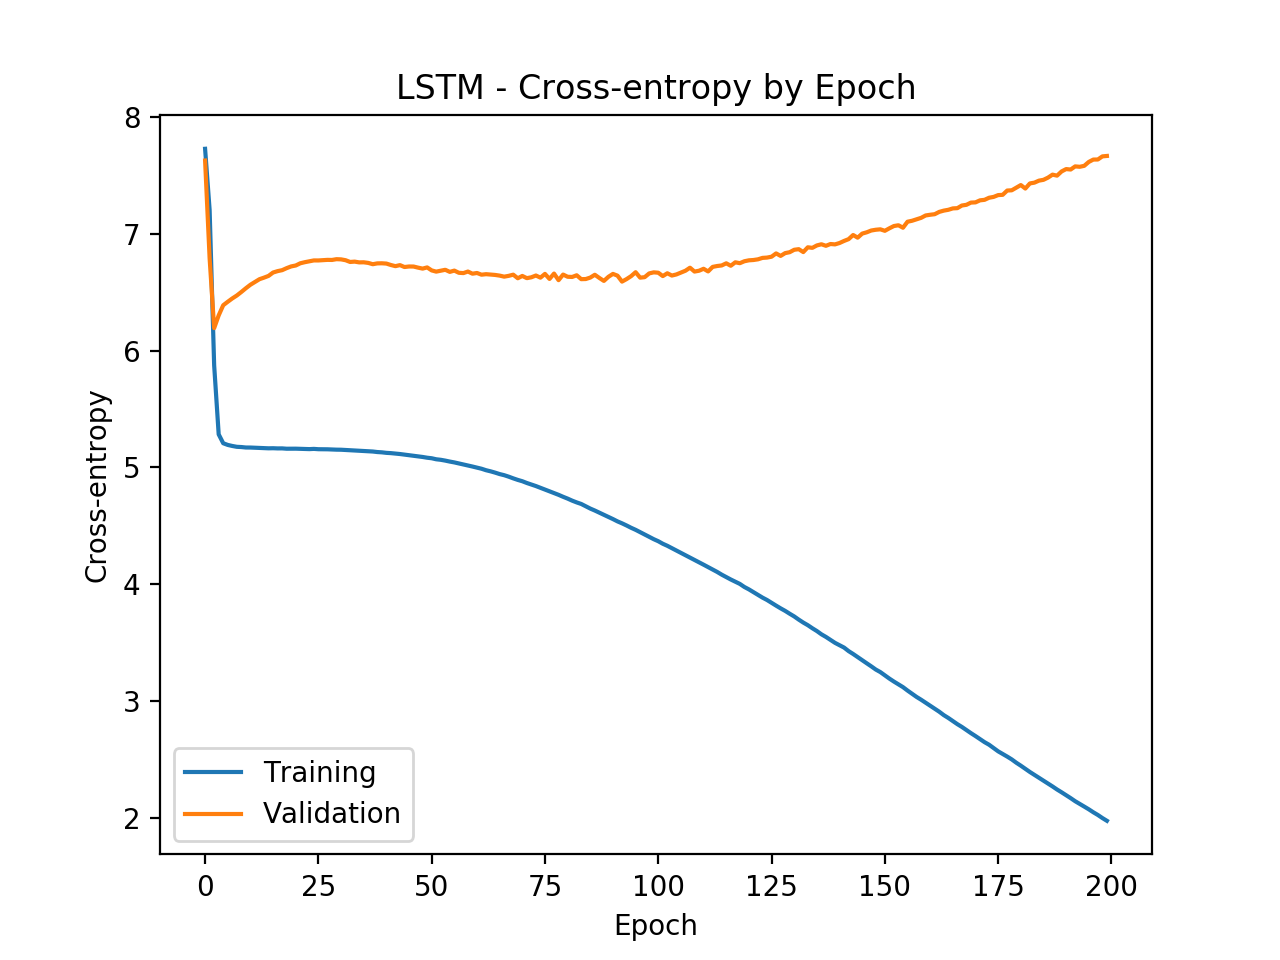
\includegraphics[width=0.5\textwidth]{LSTM_Loss.png}
    \caption{LSTM Learning Curves}
    \label{fig:LearningCurves}
\end{figure}

We direct the reader to section \ref{sec:discconc} for additional discussion and proposition for using neural model for NLG.

\subsubsection{Markov chain model}
\label{sec:markov}
Owing to the challenges in developing and training a successful neural sentence generator outlined in the previous section \ref{sec:lstm}, a model based on a popular open-source Markov chain library, \textit{markovify} \cite{markovify}, was implemented as ``Model B'' of \textit{prose2poetry}.

A Markov chain is a statistical model which computes probabilities of sequences of random variables from a set of possible values, referred to as states \cite[Chapter~8]{jurafskymarkov}. They were first used by \citet{markov} to predict whether the next letter in a sequence was a vowel or a consonant. Figure \ref{fig:markov} shows a graphic of a Markov chain for English word transitions.

\begin{figure}
	\centering
	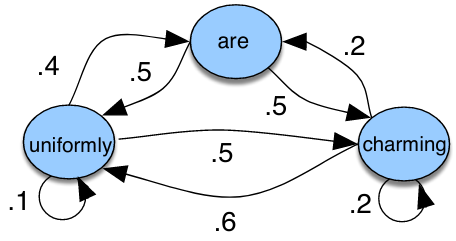
\includegraphics[scale=0.35]{./markov_chain.png}
	\caption{Illustration of Markov chain for word transition probabilities \cite{jurafskymarkov}}
\label{fig:markov}
\end{figure}

The Markov chain implementation in the \textit{markovify} library takes a corpus of sentences as an input, splits it into words, and builds probabilities of forward word transitions starting from the beginning of a sentence and moving towards the end. From this, new sentences can be generated using the observed word transition probabilities in the input corpus and a provided beginning word.

Additional work was done by \citet{markovifyfork} to implement a backwards Markov chain generator in the \textit{markovify} library. This reverses the order in which sentences from the corpus are consumed to build the model, resulting in transitions that move backwards in a sentence starting from an ending word. This is exactly suitable for the purposes of \textit{prose2poetry}, where an end word is provided as an input, and a new sentence should be generated from knowledge of the input corpus with that end word. The library also has checks to avoid exact recreations of the input text.

\subsubsection{Sentence semantic relatedness}
\label{sec:doc2vec}
As explained in \ref{sec:fasttext}, the word pairs are selected to be related in context so that the whole generated sentences are semantically related as well. 

An analysis was conducted to validate this assumptions by using a sentence embedding \cite{docvec}. For the Markov chain model, the cosine distance between the two sentence embedding vectors showed an improvement of around 10\% when evaluating 1000 generated sentences. This confirm the design choice of word pair generation.

% Markov: 0.51799 vs 0.562932 
% LSTM: 0.607907 vs 0.611643

%%%%%%%%%%%%%%
% EXP & RESULTS		%
%%%%%%%%%%%%%%
\section{Experiments and Results}
\label{sec:results}

\subsection{Baseline corpora}
\label{sec:corpora}

Using a similar approach to \citet{cole}, the Gutenberg Poetry \cite{gutenbergpoetry} and PoetryFoundation \cite{poetryfoundationkaggle} datasets were filtered to produce rhyming couplets, as its easier to extract couplets from larger poetry datasets than it is to find datasets exclusively containing couplets.

The filtering process uses the rhymes function available in the pronouncingpy library to extract every pair with rhyming end words from the same poem as a couplet. The total is 331,713 rhyming couplets from Gutenberg, and 10,009 rhyming couplets from PoetryFoundation.

\subsection{Couplet evaluation}
\label{sec:coupleteval}

A couplet scoring function was developed to evaluate the couplets. The score focuses only on the form of the couplets. This is measured with two components -- the end word rhyme score, and a stress score which measures syllabic meter \cite{meter_def}.

\subsubsection{Rhyme score}
\label{sec:rhymescore}
The rhyme score returns a real value representing the strength of the rhyme between two words. It uses phoneme data from the CMUdict in a weighted sum of three heuristic scores:
\begin{tight_itemize}
	\vspace{-0.5em}
	\item \textit{Reverse consecutive phoneme matching} (RCPM):
	RCPM counts, in reverse order starting from the end of both words, how many consecutive phoneme matches occur between the two words, normalized by the maximum possible matches. Let $c^{(a,b)}_{\text{phoneme}}$ be the reverse consecutive phoneme matches between words $a$ and $b$ and let $n^{(i)}_{\text{phoneme}}, i = {a, b}$ be the phoneme count for the words $a$ and $b$, then:
	$$\textrm{RCPM}^{(a,b)} = \frac{c^{(a,b)}_{\text{phoneme}}}{\min(n^{(a)}_{\text{phoneme}}, n^{(b)}_{\text{phoneme}})}$$
	\item \textit{Overall phoneme matching} (OPM):
		OPM counts all common phonemes between a pair of words without considering order. Let $m^{(a,b)}_{\text{phoneme}}$ be the total number of phoneme matches between word $a$ and $b$, and $n^{(i)}_{\text{phoneme}}, i = {a, b}$ be the phoneme counts for words $a$ and $b$, then:
		$$\textrm{OPM}^{(a,b)} = \frac{2 * m^{(a,b)}_{\text{phoneme}}}{n^{(a)}_{\text{phoneme}} + n^{(b)}_{\text{phoneme}}}$$
		This can be considered an adapted \citet{ratcliff} string similarity score with phonemes instead of characters.
	\item \textit{Syllable count matching} (SCM):
	The last score selects for words close in number of syllables. Let $n^{(i)}_{\text{syllable}}, i = {a, b}$ be the total counts of syllables in words $a$ and $b$.
	\begin{equation}
	\textrm{SCM}^{(a,b)} = 
	\begin{cases}
	\nonumber 1 \text{ if $\max(n^{(a)}_{\text{syllable}}, n^{(b)}_{\text{syllable}})$ = 1}\\
	\nonumber \frac{\min(n^{(a)}_{\text{syllable}}, n^{(b)}_{\text{syllable}}) - 1}{\max(n^{(a)}_{\text{syllable}}, n^{(b)}_{\text{syllable}}) - 1} \text{ otherwise}\\
        \end{cases}
	\end{equation}
	The subtraction by 1 is to ensure that the lowest possible SCM score can be 0.
\end{tight_itemize}

These are combined in a weighted average. \textcolor{red}{The weights were fine-tuned with manual tested and are shown in table \ref{table:weight_rhyme_score}}. Examples of rhyme scores are shown in the code example in figure \ref{fig:rhymescorecode}. There are some additions for special cases:
\begin{tight_enumerate}
	\vspace{-0.5em}
	\item
		Identical words have a rhyme score of 0.
	\item
		Longer rhymes score higher, up to a ceiling of 6 phonemes. Without this, single-syllable words tend to dominate the rhyme score.
	\item
		If there are multiple possible pronunciations, rhyme score returns the maximum score across all the pronunciation permutations for word $a$ and $b$, discussed further in section \ref{sec:synset}.
\end{tight_enumerate}

\begin{table}[ht]
\centering
\begin{tabular}{lll c c c}
	\hline\hline
	RCPM & OPM & SCM \\ [0.5ex]
	\hline\hline
	34\% & 33\% & 33\% \\ [0.5ex]
	\hline
\end{tabular}
\caption{Weights of rhyme score}
\label{table:weight_rhyme_score}
\end{table}

\begin{figure}
\begin{Verbatim}[fontsize=\small]
>>> rhyme_score('affection', 'perfection')
0.88
>>> rhyme_score('affection', 'disgust')
0.075
\end{Verbatim}
\caption{Some examples of rhyme score}
\label{fig:rhymescorecode}
\end{figure}

\subsubsection{Meter score}
\label{sec:stressscore}

Using the pronouncingpy library, the syllabic stress of all of the words in each line is concatenated to represent the syllabic meter \cite{meter_def} of each sentence. In the CMUdict, 0 represents an unstressed syllable, 1 represents primary stress, and 2 represents secondary stress.  Examples are shown in table \ref{table:stress}. The \citet{ratcliff} string similarity score is then applied on the concatenated stress strings of the two sentences in the couplet.

\begin{table}
\centering
\begin{tabular}{ll c c}
	\hline\hline
	Sentence & Stress \\ [0.5ex]
	\hline\hline
	He likes jam & 111 \\ [0.5ex]
	\hline
	She likes ham & 111 \\ [0.5ex]
	\hline
	Alexander the Great conquered & 20100110 \\ [0.5ex]
	\hline
\end{tabular}
\caption{Cases of matched and mismatched stress strings for comparing meter}
\label{table:stress}
\end{table}

\subsubsection{Couplet score}
\label{sec:coupletscore}

The total couplet score is a weighted sum of the two metrics above, resulting in a single real value $\in [0, 1]$. \textcolor{red}{The weights assigned to each score were again fine-tuned with manual adjustment, leading to the final weights in table \ref{table:weight_couplet_score}.}

\begin{table}[ht]
\centering
\begin{tabular}{lll c c c}
	\hline\hline
	Rhyme & Meter \\ [0.5ex]
	\hline\hline
	50\% & 50\% \\ [0.5ex]
	\hline
\end{tabular}
\caption{Weights of couplet score}
\label{table:weight_couplet_score}
\end{table}

It was mentioned that the couplet score is focused on form only, and not couplet contents. This can be problematic -- consider the example ``ham ham ham, jam jam jam.'' This couplet has a nearly perfect score of 0.89 (out of 1.0) since it rhymes and has exactly matching meter. However, a human judge wouldn't rate it as good poetry. There were many challenges involved in evaluating the semantic coherence, grammatical correctness, or other aspects of the contents of the couplets. These are discussed in section \ref{sec:discconc}.

\textcolor{red}{
REMOVE NAIVE GENERATOR FROM SCORE TABLE + REMOVE NAIVE FROM EXAMPLE + KEEP ONLY ONE POEM FOR EXAMPLE
}
\begin{table*}[ht]
\begin{tabular}{|l|l|l|l|l|l|l|l|l|l|l|c|c|c|c|c|c|c|c|c|c|}
\hline\hline
\multicolumn{1}{|c|}{Score} & \multicolumn{3}{c|}{Couplet} & \multicolumn{3}{c|}{Rhyme} & \multicolumn{3}{c|}{Meter}\\
\cline{1-10}
\multicolumn{1}{|c|}{Dataset} & Mean & SD & .95q & Mean & SD & .95q & Mean & SD & .95q \\
\hline\hline
Gutenberg & 0.69 & 0.12 & 0.86 & 0.70 & 0.18 & 0.93 & 0.68 & 0.14 & 0.89 \\ [0.5ex]
\hline
PoetryFoundation & 0.68 & 0.12 & 0.85 & 0.70 & 0.19 & 0.93 & 0.68 & 0.14 & 0.89 \\ [0.5ex]
\hline
\textit{prose2poetry} LSTM & 0.59 & 0.12 & 0.78 & 0.68 & 0.17 & 0.91 & 0.50 & 0.19 & 0.80 \\ [0.5ex]
\hline
\textit{prose2poetry} Markov chain & 0.58 & 0.12 & 0.77 & 0.68 & 0.17 & 0.90 & 0.47 & 0.19 & 0.77 \\ [0.5ex]
\hline
Naive generator & 0.57 & 0.15 & 0.79 & 0.66 & 0.18 & 0.93 & 0.48 & 0.21 & 0.80 \\ [0.5ex]
\hline
Prose & 0.33 & 0.13 & 0.56 & 0.19 & 0.18 & 0.46 & 0.48 & 0.19 & 0.76 \\ [0.5ex]
\hline
\end{tabular}

\caption{Couplet scores of \textit{prose2poetry} generated outputs and baselines}
\label{table:couplet_results}
\end{table*}

\begin{table*}[ht]
\begin{tabular*}{\textwidth}{ll cc}
	\hline\hline
	Source & Couplets \\ [0.5ex]
	\hline\hline
	Gutenberg baseline & \makecell[l] {(`The vision came and went', `The light shone and was spent')\\(`Close your little gap he hitches', `Whistlin' as he jabs the stitches') } \\ [0.5ex]
	\hline
	PoetryFoundation baseline & \makecell[l]{(`Tells himself that he tried', `Tells himself that he cried and cried')\\(`Much mirth and no madness', `All good and no badness') } \\ [0.5ex]
	\hline
	Prose & \makecell[l]{(`the mistake had been slight', `the carriage was sent for them now')\\(`i give you credit for it', 'this is feeling your way')} \\ [0.5ex]
	\hline
	Naive generator & \makecell[l]{(`regular features , open countenance , with a complexion',\\`this was the conclusion of the first series of reflection')\\(`do not be overpowered by such a little tribute of admiration',\\`she then took a longer time for consideration')} \\ [0.5ex]
	\hline
	\textit{prose2poetry} Markov chain & \makecell[l]{(`And I hate Italian singing', `It must have penetrated a part in bringing')\\(`I could never see a better', `I hope , a highly prized letter')} \\ [-1.5ex]
	\hline
	\textit{prose2poetry} LSTM & \makecell[l]{(`had her neighborhood drinking', `though her sinking')\\(`he had now required', `would be who retired')} \\ [0.5ex]
	\hline
\end{tabular*}
\caption{Examples of top-scoring couplets from all evaluated datasets}
\label{table:bestcouplets}
\end{table*}

\subsection{Results}
\label{sec:results}
\subsubsection{Quantitative assessment}

The results in table \ref{table:couplet_results} were evaluated on 1,000 couplets randomly selected from the baselines and \textit{prose2poetry} generator models. These were selected to be a representative sample from the larger datasets. The evaluation was repeated with different RNG seeds, observing that different random selections of couplets from the same source tended to have a stable score.

The prose baseline was created by selecting random sentence pairs from the input English novel corpus without any filtering. \textcolor{red}{The naive generator created couplets by finding and returning sentences in the input corpus that rhyme using prouncingpy.}

The total couplet score is shown, as well as each of the subcomponents for further discussion. The mean, standard deviation, and .95 quantile were chosen as statistical metrics for the scores.

\subsubsection{Qualitative assessment}

From each evaluated dataset, two couplets which scored better than the .95 quantile score are included in table \ref{table:bestcouplets} for the readers to enjoy and judge for themselves.

%%%%%%%%%%%%%%
% DISC & CONC		%
%%%%%%%%%%%%%%
\section{Discussion and conclusion}
\label{sec:discconc}

\textcolor{green}{
Results interpretation here. "Our poems scored well, stress score showed real poems have good meter, etc."
}

\textcolor{Orchid}{
\subsection{Sevag discussion/conclusion ideas}
sevag ideas
}

\subsection{Francois discussion/conclusion ideas}
The trained LSTM explained in section \ref{sec:lstm} did not perform to expected standard. One possible improvement would have been to use pre-trained model like GPT-2 \cite{gpt2} with flavor of our prose corpus. Using additional corpus would have been against the spirit of our project goal and not a possible avenue.

\subsection{Multiple pronunciations and sense disambiguation}
\label{sec:synset}

Difficulty was encountered in the rhyme score when trying to associate different pronunciations of homographs with their respective senses or parts of speech. \textcolor{red}{\citet{hopkins-kiela-2017} state that:
\begin{quote}
Pronunciation dictionaries have often been used to determine the syllabic stresses of words, but suffer from some limitations [...]. All word pronunciations are considered equiprobable, including archaic and uncommon pronunciations, and pronunciations are provided context free, despite the importance of context for pronunciation.
\end{quote}}

Consider two examples, using WordNet \cite{wordnet} as a lexical resource via NLTK:
\begin{tight_enumerate}
	\vspace{-0.5em}
	\item
		In the CMUdict, there are two pronunciations for ``bow'': like ``cow'' or like ``snow''. In WordNet, there are fourteen synsets for ``bow'', and two different parts of speech.
	\item
		In the CMUdict, there are two pronuncations for ``defect'': noun with beginning emphasis ``DEE-fect'', or verb with end emphasis ``de-FECT''. In WordNet, there are five synsets for ``defect'', and two different parts of speech.
\end{tight_enumerate}

There is no readily available mapping between CMUdict pronunciation and WordNet senses. This can only be resolved with a lexical resource that provides combined sense and pronunciation disambiguation -- Wiktionary \cite{wiktionary} is one such option, but scraping it was considered beyond the scope of this paper. The final approach chosen was to ignore ambiguity and return the best rhyme score across all possible pronunciation permutations.

\textcolor{Orchid}{
\subsection{Couplet content evaluation}
\label{sec:nlg}
difficulty with NLG, METEOR, BERT next sentence prediction, grammatical content
}

\textcolor{Orchid}{
\subsection{Code availability}
Describe open source code location, GitHub link, package structure (very brief), etc.
}

%%%%%%%%%%%%%%
% STAT OF CONT		%
%%%%%%%%%%%%%%
\section{Statement of contributions}
\label{sec:contributions}
Sevag Hanssian worked on finding different poem baselines \& the prose dataset, creating the coding architecture, developing the couplet scoring and running the experiments. François Milot developed the word embedding (FastText), the doc2vec training, the word pair generation and design of the rhyme score. Also, the design and direction of the project have been decided as a group. 

\bibliographystyle{acl_natbib}
\bibliography{final_report}

\end{document}
